\documentclass[grado3]{LEMA-Tikz-IM}

\usepackage{graphicx}  % Needed to include graphics
\usepackage{pifont} % For the scissors symbol

\begin{document}
\begin{tikzpicture}
% \pgfplotsset{compat=1.18}

% page canvas letter size
\path (0,0) rectangle (8.5in,11in);

\def\myMargin{1in}

\coordinate (botLeft) at (\myMargin,\myMargin);
\coordinate (botRight) at (8.5in-\myMargin,\myMargin);
\coordinate (topRight) at (8.5in-\myMargin,11in-\myMargin);
\coordinate (topLeft) at (\myMargin,11in-\myMargin);

% clip outside the margin 
% \draw (botLeft) rectangle (topRight);


% find center of printable page
\coordinate (centerTop) at ($ (topLeft)!0.5!(topRight) $);

% add tables to top and bottom
\node[anchor=north] (table1) at ([yshift=-8ex]centerTop) {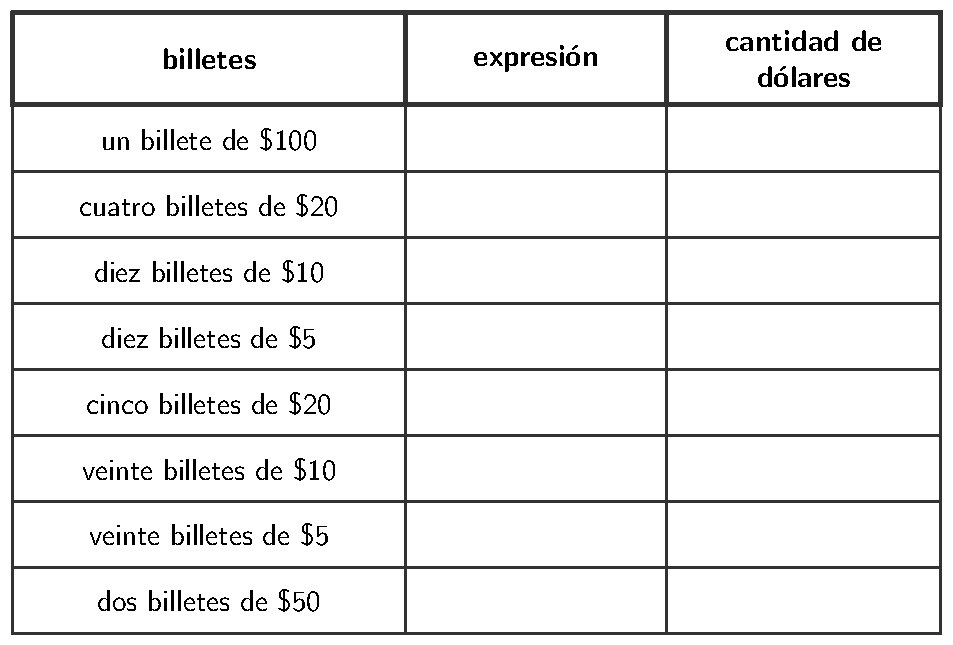
\includegraphics[scale=0.95]{unaGranCantidadDeDolares-blm-tab1.pdf}};
\node[anchor=north] (table2) at ([yshift=-3ex]table1.south) {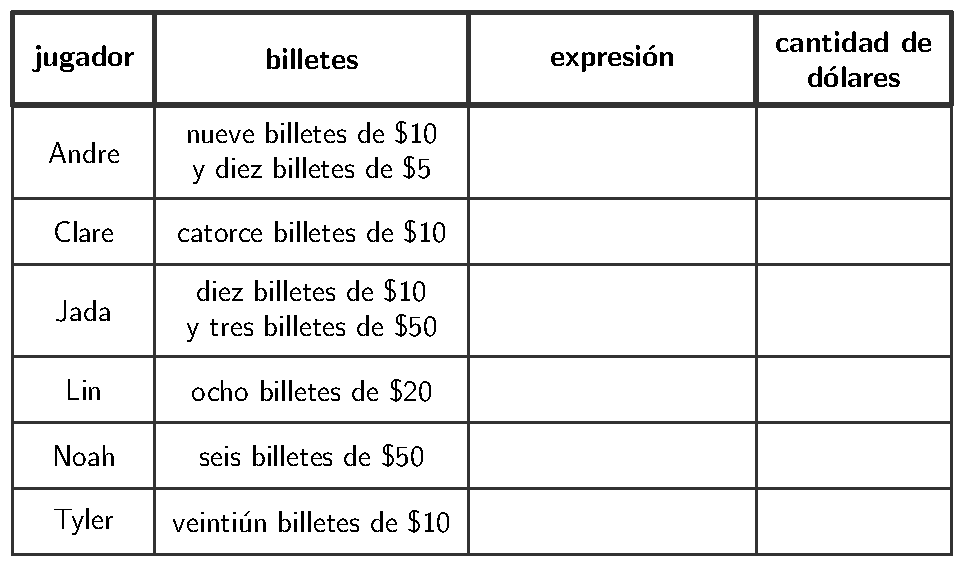
\includegraphics[scale=0.95]{unaGranCantidadDeDolares-blm-tab2.pdf}};


% Add BLM heading to top and bottom
\node[below right, align=left, font=\bf] at (topLeft) {\Large Una gran cantidad de dólares};


% Espacio de nombre
\node[below left] at ([yshift=6ex]topRight) {Nombre: \underline{\hspace{6cm}}};


\end{tikzpicture}
\end{document}